\documentclass[12pt,a4paper]{article}

% ── Fonts & Encoding ─────────────────────────────────────────────
\usepackage[T1]{fontenc}
\usepackage[utf8]{inputenc}
\usepackage{mathptmx}          % Times New Roman
\usepackage{microtype}

% ── Page Layout ──────────────────────────────────────────────────
\usepackage[
  top=2.5cm, bottom=2.5cm,
  left=3cm,  right=2.5cm
]{geometry}

% ── Line Spacing ─────────────────────────────────────────────────
\usepackage{setspace}
\setstretch{1.5}

% ── Colors ───────────────────────────────────────────────────────
\usepackage{xcolor}
\definecolor{iiucblue}{RGB}{0,51,102}
\definecolor{codeblue}{RGB}{30,100,180}
\definecolor{codegray}{RGB}{245,245,245}
\definecolor{codecomment}{RGB}{80,120,80}

% ── Graphics & Tables ────────────────────────────────────────────
\usepackage{graphicx}
\usepackage{booktabs}
\usepackage{array}
\usepackage{tabularx}

% ── Code Listings ────────────────────────────────────────────────
\usepackage{listings}
\lstdefinestyle{cppstyle}{
  language=C++,
  backgroundcolor=\color{codegray},
  basicstyle=\ttfamily\footnotesize,
  keywordstyle=\color{codeblue}\bfseries,
  commentstyle=\color{codecomment}\itshape,
  stringstyle=\color{red!60!black},
  numberstyle=\tiny\color{gray},
  numbers=left,
  numbersep=8pt,
  frame=single,
  framerule=0.4pt,
  rulecolor=\color{gray!50},
  breaklines=true,
  showstringspaces=false,
  tabsize=4,
  xleftmargin=12pt,
  aboveskip=6pt,
  belowskip=6pt,
  abovecaptionskip=4pt,
}
\lstdefinestyle{nestyle}{
  language={},
  backgroundcolor=\color{codegray},
  basicstyle=\ttfamily\footnotesize,
  keywordstyle=\color{codeblue}\bfseries,
  morekeywords={simple,network,submodules,connections,gates,parameters,
                inout,default,packet,int,output,input,numPackets},
  commentstyle=\color{codecomment}\itshape,
  morecomment=[l]{//},
  numbers=left,
  numberstyle=\tiny\color{gray},
  numbersep=8pt,
  frame=single,
  framerule=0.4pt,
  rulecolor=\color{gray!50},
  breaklines=true,
  showstringspaces=false,
  tabsize=4,
  xleftmargin=12pt,
  aboveskip=6pt,
  belowskip=6pt,
}
\lstdefinestyle{inistyle}{
  language={},
  backgroundcolor=\color{codegray},
  basicstyle=\ttfamily\footnotesize,
  morecomment=[l]{\#},
  commentstyle=\color{codecomment}\itshape,
  numbers=left,
  numberstyle=\tiny\color{gray},
  numbersep=8pt,
  frame=single,
  framerule=0.4pt,
  rulecolor=\color{gray!50},
  breaklines=true,
  showstringspaces=false,
  tabsize=4,
  xleftmargin=12pt,
  aboveskip=6pt,
  belowskip=6pt,
}
\lstdefinestyle{pystyle}{
  language=Python,
  backgroundcolor=\color{codegray},
  basicstyle=\ttfamily\footnotesize,
  keywordstyle=\color{codeblue}\bfseries,
  commentstyle=\color{codecomment}\itshape,
  stringstyle=\color{red!60!black},
  numbers=left,
  numberstyle=\tiny\color{gray},
  numbersep=8pt,
  frame=single,
  framerule=0.4pt,
  rulecolor=\color{gray!50},
  breaklines=true,
  showstringspaces=false,
  tabsize=4,
  xleftmargin=12pt,
  aboveskip=6pt,
  belowskip=6pt,
}

% ── TikZ ─────────────────────────────────────────────────────────
\usepackage{tikz}
\usetikzlibrary{shapes.geometric, arrows.meta, positioning, calc}

% ── Headers & Footers ────────────────────────────────────────────
\usepackage{fancyhdr}
\pagestyle{fancy}
\fancyhf{}
\fancyhead[L]{\small\textcolor{iiucblue}{CSE-4834: Computer Networks Lab}}
\fancyhead[R]{\small\textcolor{iiucblue}{Lab Report: Hop Counting}}
\fancyfoot[C]{\small\thepage}
\renewcommand{\headrulewidth}{0.4pt}
\renewcommand{\headrule}{\hbox to\headwidth{\color{iiucblue}\leaders\hrule height \headrulewidth\hfill}}

% ── Misc ─────────────────────────────────────────────────────────
\usepackage{parskip}
\setlength{\parindent}{0pt}
\setlength{\parskip}{4pt}
\usepackage{enumitem}
\setlist[itemize]{noitemsep, topsep=2pt, leftmargin=20pt}
\setlist[enumerate]{noitemsep, topsep=2pt, leftmargin=20pt}
\usepackage{hyperref}
\hypersetup{colorlinks=true, linkcolor=iiucblue, urlcolor=iiucblue}
\usepackage{tcolorbox}
\tcbuselibrary{skins,breakable}
\usepackage{caption}
\captionsetup{font=small, labelfont=bf}
\usepackage{float}
\usepackage{amsmath}
\usepackage{ragged2e}

% ── Font Sizes ───────────────────────────────────────────────────
\usepackage{sectsty}
\sectionfont{\fontsize{16}{20}\selectfont\color{iiucblue}\bfseries}
\subsectionfont{\fontsize{14}{18}\selectfont\color{iiucblue}\bfseries}
\subsubsectionfont{\fontsize{12}{16}\selectfont\bfseries}



% ─────────────────────────────────────────────────────────────────
%  DOCUMENT
% ─────────────────────────────────────────────────────────────────
\begin{document}
\thispagestyle{empty}

% ══════════════════════════════════════════════════════════════════
%  COVER PAGE
% ══════════════════════════════════════════════════════════════════
\begin{center}
\includegraphics[width=0.4\textwidth]{screenshot/bismillah.png}

{\fontsize{15}{18}\selectfont\bfseries\textcolor{iiucblue}{%
Bachelor of Science in Computer Science \& Engineering}}

\vspace{0.1cm}
{\fontsize{11}{13}\selectfont CSE-3634, Computer Networks Lab}

\noindent\textcolor{iiucblue}{\rule{\linewidth}{0.8pt}}

{\fontsize{15}{18}\selectfont\bfseries\underline{Lab Report: 04}}

\vspace{0.2cm}

{\fontsize{15}{18}\selectfont\bfseries\underline{Hop Counting in Random Mesh Network}} \\[2pt]
{\fontsize{15}{18}\selectfont\bfseries\underline{Using OMNeT++ Simulation}}

\vspace{0.1cm}
\noindent\textcolor{iiucblue}{\rule{\linewidth}{0.8pt}}

\vspace{0.5cm}

{\fontsize{13}{15}\selectfont\bfseries\underline{Submitted by}}

\vspace{0.2cm}
{\fontsize{11}{13}\selectfont
Umme Benin Yeasmin Meem (C231452)\\
Kazi Namira Meyheg Sanam (C231450)\\
Semester: 7BF}

\vspace{0.5cm}

{\fontsize{13}{15}\selectfont\bfseries\underline{Submitted to}}

\vspace{0.2cm}
{\fontsize{11}{13}\selectfont
Nourin Noushrat Noushin\\
Lecturer, Dept of CSE, IIUC}

\vspace{0.6cm}

{\small Combines Quality With Morality}

\vspace{0.2cm}

\includegraphics[width=2.5cm]{iiuc_logo.png}

{\small Estd. February 11, 1995}

\vspace{0.5cm}

{\fontsize{13}{15}\selectfont\bfseries\textcolor{iiucblue}{%
Department of Computer Science \& Engineering}}

{\fontsize{11}{13}\selectfont
International Islamic University Chittagong, Bangladesh}

\vspace{0.2cm}
{\fontsize{11}{13}\selectfont\bfseries\textcolor{iiucblue}{9 May, 2026}}

\end{center}

\newpage

% ══════════════════════════════════════════════════════════════════
%  TABLE OF CONTENTS
% ══════════════════════════════════════════════════════════════════
\tableofcontents
\newpage

% ══════════════════════════════════════════════════════════════════
%  SECTION 1 — INTRODUCTION
% ══════════════════════════════════════════════════════════════════
\section{Introduction:}

\justifying
In modern computer networks, data packets travel through multiple intermediate nodes (routers) before reaching their final destination. The number of routers a packet passes through is commonly referred to as the \textbf{hop count}. Understanding and analyzing hop counts is fundamental to network performance evaluation, routing optimization, and Quality of Service (QoS) management. A \textbf{mesh network} is a topology where each node (router) is connected to multiple other nodes, creating several alternative paths between any source and destination. This redundancy increases network reliability but also introduces variability in routing behavior, especially when random routing decisions are applied at each node. This lab investigates how packets traverse a randomly connected mesh network of ten routers using \textbf{OMNeT++}, a widely-used discrete-event network simulator. The simulation network consists of 12 nodes in total: 1 Sender, 10 Routers (r0--r9), and 1 Receiver. Each router forwards arriving packets to a randomly selected connected neighbor, and a Time-To-Live (TTL) mechanism is enforced to prevent infinite routing loops. By executing six independent simulation runs with different random seeds, the distribution of hop counts is observed, analyzed, and visualized to understand how routing randomness affects packet traversal path length in a mesh topology.

% ══════════════════════════════════════════════════════════════════
%  SECTION 2 — OBJECTIVES
% ══════════════════════════════════════════════════════════════════
\section{Objectives: }

\justifying
The objectives of this laboratory experiment are as follows:

\begin{itemize}
  \item To design and implement a random mesh network topology with 10 routers in OMNeT++ using the NED language.
  \item To define a custom message type (\texttt{MyMessage}) carrying \texttt{hopCount} and \texttt{ttl} integer fields.
  \item To implement hop counting logic where each router increments \texttt{hopCount} by one each time a packet passes through it.
  \item To implement a TTL-based packet drop mechanism that prevents routing loops and limits packet lifetime in the network.
  \item To simulate random routing by forwarding packets to a uniformly randomly selected outgoing gate at every router.
  \item To execute six independent simulation runs using different random seeds (42, 100, 255, 777, 1234, 9999).
  \item To record the final \texttt{hopCount} value at the Receiver for each simulation run and compute statistical results.
  \item To analyze and visualize the distribution of hop counts and packet delivery/drop statistics using a Python script.
\end{itemize}

% ══════════════════════════════════════════════════════════════════
%  SECTION 3 — PROBLEM STATEMENT
% ══════════════════════════════════════════════════════════════════
\section{Problem Statement: }

\subsection*{Given:}
\justifying
A mesh network of 10 routers connecting a Sender host and a Receiver host. The network uses random routing, where each router forwards an incoming packet to one of its connected neighbors selected uniformly at random. The Sender generates 50 packets, each initialized with \texttt{hopCount = 0} and \texttt{ttl = 20}.

\subsection*{Required:}
\begin{enumerate}
  \item Build a mesh network with 10 routers in OMNeT++ using the NED topology description language.
  \item Define a custom packet (\texttt{MyMessage}) with two integer fields: \texttt{hopCount} (initialized to 0) and \texttt{ttl} (initialized to 20).
  \item At each router:
  \begin{itemize}
    \item Increment \texttt{hopCount} by 1.
    \item Decrement \texttt{ttl} by 1; drop the packet if \texttt{ttl} reaches zero.
    \item Forward the packet to a randomly chosen connected output gate.
  \end{itemize}
  \item Run 6 simulations with different seeds and record the \texttt{hopCount} at the Receiver for each received packet.
  \item Compute the average hop count per run and overall, then plot the distribution.
\end{enumerate}
% ══════════════════════════════════════════════════════════════════
%  SECTION 4 — THEORY
% ══════════════════════════════════════════════════════════════════
\section{Theory: }

\subsection{Hop Count: }

\justifying
The \textbf{hop count} of a packet is defined as the number of intermediate network devices (routers or switches) the packet traverses from its source to its destination. Formally, if a packet visits nodes $v_0 \to v_1 \to v_2 \to \cdots \to v_k$, where $v_0$ is the Sender and $v_k$ is the Receiver, the hop count equals $k$. A lower hop count generally indicates a shorter, more efficient path through the network.

\subsection{Time To Live (TTL): }

\justifying
\textbf{TTL} is a field embedded in the packet header that limits the packet's lifetime within the network. At each hop, the forwarding router decrements TTL by 1. When TTL reaches zero, the packet is discarded. This mechanism prevents routing loops from indefinitely consuming network resources. The mathematical formulation is:

\[
\text{TTL}_{n+1} = \text{TTL}_{n} - 1 \qquad \text{drop if } \text{TTL}_{n+1} \leq 0
\]

\subsection{Random Routing: }

\justifying
In random routing, a router selects the next hop uniformly at random from its set of connected neighbors. If a router has $d$ connected output gates, each gate is selected with probability $\frac{1}{d}$. This produces variable path lengths across different simulation runs, reflecting the stochastic nature of the routing process and resulting in a distribution of hop counts rather than a fixed value.

\subsection{Mesh Network Topology:}

\justifying
A mesh network provides multiple paths between any source-destination pair. The number of possible paths grows combinatorially with network size and connectivity. In the topology used in this lab, the routers are organized with dense interconnections, giving each router several forwarding choices. This rich connectivity ensures packets are seldom dropped due to dead ends and makes the simulation representative of realistic mesh network behavior.

% ══════════════════════════════════════════════════════════════════
%  SECTION 5 — NETWORK DESIGN
% ══════════════════════════════════════════════════════════════════
\section{Network Design: }

\subsection{Topology Overview:}

\justifying
The simulation network consists of \textbf{12 nodes}: 1 Sender, 10 Routers (r0--r9), and 1 Receiver. The routers form a directed mesh where each router maintains multiple outgoing connections to neighboring routers, creating diverse forwarding paths. The topology is defined using OMNeT++'s NED language with unidirectional \texttt{output} and \texttt{input} gates with auto-indexed (\texttt{++}) gate arrays.

\begin{figure}[H]
\centering
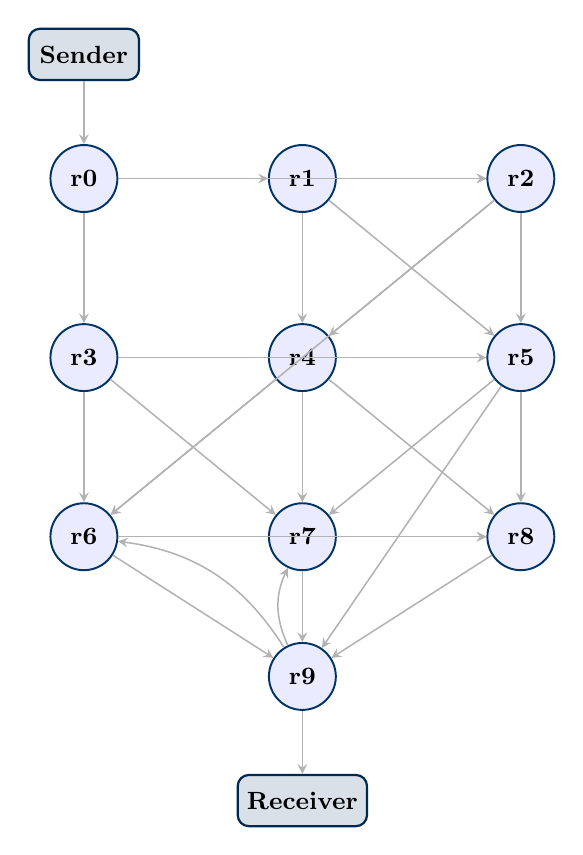
\begin{tikzpicture}[
  node distance=1.4cm and 1.9cm,
  router/.style={circle, draw=iiucblue, fill=blue!8, minimum size=0.85cm,
                 font=\small\bfseries, line width=0.7pt},
  host/.style={rectangle, rounded corners=4pt, draw=iiucblue!80!black,
               fill=iiucblue!15, minimum width=1.4cm, minimum height=0.65cm,
               font=\small\bfseries, line width=0.8pt},
  fwd/.style={->, gray!60, line width=0.55pt, >=stealth},
]

% Nodes
\node[host] (sender) {Sender};
\node[router, below=0.8cm of sender] (r0) {r0};
\node[router, right=of r0] (r1) {r1};
\node[router, right=of r1] (r2) {r2};
\node[router, below=of r0] (r3) {r3};
\node[router, right=of r3] (r4) {r4};
\node[router, right=of r4] (r5) {r5};
\node[router, below=of r3] (r6) {r6};
\node[router, right=of r6] (r7) {r7};
\node[router, right=of r7] (r8) {r8};
\node[router, below=0.9cm of r7] (r9) {r9};
\node[host, below=0.8cm of r9] (recv) {Receiver};

% Edges (directed)
\draw[fwd] (sender) -- (r0);
\draw[fwd] (r0) -- (r1); \draw[fwd] (r0) -- (r2); \draw[fwd] (r0) -- (r3);
\draw[fwd] (r1) -- (r4); \draw[fwd] (r1) -- (r5); \draw[fwd] (r1) -- (r2);
\draw[fwd] (r2) -- (r4); \draw[fwd] (r2) -- (r6); \draw[fwd] (r2) -- (r5);
\draw[fwd] (r3) -- (r5); \draw[fwd] (r3) -- (r7); \draw[fwd] (r3) -- (r6);
\draw[fwd] (r4) -- (r6); \draw[fwd] (r4) -- (r8); \draw[fwd] (r4) -- (r7);
\draw[fwd] (r5) -- (r7); \draw[fwd] (r5) -- (r8); \draw[fwd] (r5) -- (r9);
\draw[fwd] (r6) -- (r8); \draw[fwd] (r6) -- (r9);
\draw[fwd] (r7) -- (r9); \draw[fwd] (r7) -- (r8);
\draw[fwd] (r8) -- (r9);
\draw[fwd] (r9) -- (recv);
\draw[fwd,bend right=25] (r9) to (r6);
\draw[fwd,bend left=25] (r9) to (r7);

\end{tikzpicture}
\caption{Directed mesh network topology: Sender $\to$ r0--r9 $\to$ Receiver}
\label{fig:topology}
\end{figure}

\justifying
This figure shows the complete directed mesh topology. The Sender connects to r0, which then fans out to r1, r2, and r3. Each intermediate router has three to four outgoing connections. The Receiver collects packets arriving from r9. Notably, r9 also connects back to r6 and r7, which introduces cycles in the directed graph and increases the variance of hop counts across runs.

\subsection{Node Roles: }

\begin{table}[H]
\centering
\renewcommand{\arraystretch}{1.4}
\begin{tabular}{@{}lll@{}}
\toprule
\textbf{Node} & \textbf{Type} & \textbf{Role} \\
\midrule
\texttt{sender}   & Sender   & Generates 50 packets at \texttt{t=0}, sends to r0 \\
\texttt{r0--r9}   & Router   & Increments hopCount, decrements TTL, random forward \\
\texttt{receiver} & Receiver & Records final hopCount and statistics \\
\bottomrule
\end{tabular}
\caption{Node types and roles in the simulation}
\end{table}

% ══════════════════════════════════════════════════════════════════
%  SECTION 6 — METHODOLOGY
% ══════════════════════════════════════════════════════════════════
\section{Methodology: }

\justifying
The lab follows a structured six-step methodology:

\begin{enumerate}
  \item \textbf{Network Setup:} A mesh network of 12 nodes is defined in OMNeT++ using the NED language. Unidirectional \texttt{input} and \texttt{output} gates with the \texttt{++} auto-indexing notation are used to create flexible gate arrays for each router.

  \item \textbf{Message Definition:} A custom \texttt{MyMessage} packet is defined in a \texttt{.msg} file with two integer fields: \texttt{hopCount} (default 0) and \texttt{ttl} (default 20). OMNeT++ auto-generates the corresponding C++ accessor methods.

  \item \textbf{Hop Counting Logic:} Each router, upon receiving a packet, increments \texttt{hopCount} by 1 and decrements \texttt{ttl} by 1. If \texttt{ttl} reaches zero, the packet is dropped and recorded as a lost packet.

  \item \textbf{Random Routing:} Each router determines the number of connected output gates (\texttt{gateSize("out")}), then uses OMNeT++'s \texttt{intuniform()} function to select a random gate index. Different \texttt{seed-set} values in \texttt{omnetpp.ini} produce different routing paths per run.

  \item \textbf{Simulation Execution:} Six independent runs (Run1--Run6) are executed with seed values 42, 100, 255, 777, 1234, and 9999. The Receiver records \texttt{hopCount} statistics and the Receiver logs all arriving packet details.

  \item \textbf{Result Analysis:} A Python script (\texttt{analyze\_results.py}) reads scalar result files, computes statistics (average, min, max, standard deviation, dropped count), and generates a 3-panel visualization chart.
\end{enumerate}

\subsection{Algorithm / Working Procedure: }


\begin{enumerate}[label=\textbf{Step \arabic*.}, leftmargin=*, noitemsep]
  \item Receive \texttt{MyMessage} packet on any input gate.
  \item Increment: \texttt{hopCount = hopCount + 1}
  \item Decrement: \texttt{ttl = ttl - 1}
  \item \textbf{If} \texttt{ttl} $\leq$ 0:
    \begin{itemize}
      \item Log: ``TTL expired -- dropping packet''
      \item Increment local \texttt{droppedCount} counter
      \item Delete packet and return (STOP)
    \end{itemize}
  \item Determine \texttt{numOut = gateSize("out")}
  \item \textbf{If} \texttt{numOut == 0}: drop packet and return (STOP)
  \item Select: \texttt{chosen = intuniform(0, numOut - 1)}
  \item Forward packet via \texttt{send(pkt, "out", chosen)}
\end{enumerate}


% ══════════════════════════════════════════════════════════════════
%  SECTION 7 — CODE
% ══════════════════════════════════════════════════════════════════
\section{Code: }

\subsection{Message Structure --- \texttt{MyMessage.msg}: }

\begin{lstlisting}[style=cppstyle, caption={MyMessage.msg -- Custom packet definition}]
// MyMessage.msg
// Custom message carrying hopCount and TTL fields

packet MyMessage
{
    int hopCount = 0;   // incremented by each router
    int ttl      = 20;  // decremented by each router; drop at 0
    int messageId = 0;  // packet sequence identifier
}
\end{lstlisting}

\justifying
OMNeT++ compiles this \texttt{.msg} file to automatically generate \texttt{MyMessage\_m.h} and \texttt{MyMessage\_m.cc}, providing getter and setter accessor methods: \texttt{getHopCount()}, \texttt{setHopCount()}, \texttt{getTtl()}, \texttt{setTtl()}, and \texttt{getMessageId()}.
\vspace{1cm}

\subsection{Sender Module --- \texttt{Sender.h} and \texttt{Sender.cc}: }

\begin{lstlisting}[style=cppstyle, caption={Sender.h -- Header file}]
// Sender.h
#ifndef __SENDER_H_
#define __SENDER_H_

#include <omnetpp.h>
#include "MyMessage_m.h"
using namespace omnetpp;

class Sender : public cSimpleModule {
  private:
    int totalPackets;
    int sentCount;
    cMessage *sendTimer;
  protected:
    virtual void initialize() override;
    virtual void handleMessage(cMessage *msg) override;
    virtual void finish() override;
};

#endif
\end{lstlisting}

\begin{lstlisting}[style=cppstyle, caption={Sender.cc -- Implementation}]
// Sender.cc
// Sends 50 packets one by one with a 0.1s interval between each.

#include "Sender.h"
Define_Module(Sender);

void Sender::initialize()
{
    totalPackets = par("numPackets");
    sentCount    = 0;
    sendTimer    = new cMessage("sendTimer");
    scheduleAt(simTime(), sendTimer);
}

void Sender::handleMessage(cMessage *msg)
{
    if (msg == sendTimer) {
        if (sentCount < totalPackets) {
            sentCount++;
            MyMessage *pkt = new MyMessage("DataPacket");
            pkt->setHopCount(0);
            pkt->setTtl(20);
            pkt->setMessageId(sentCount);
            EV << "[Sender] Sending packet #" << sentCount
               << " hopCount=0 ttl=20\n";
            send(pkt, "out");
            scheduleAt(simTime() + 0.1, sendTimer);
        } else {
            EV << "[Sender] All " << totalPackets
               << " packets sent.\n";
            delete sendTimer;
            sendTimer = nullptr;
        }
    } else {
        delete msg;
    }
}

void Sender::finish()
{
    EV << "[Sender] Total packets sent: " << sentCount << "\n";
}
\end{lstlisting}

\subsection{Router Module --- \texttt{Router.h} and \texttt{Router.cc}: }

\begin{lstlisting}[style=cppstyle, caption={Router.h -- Header file}]
// Router.h
#ifndef __ROUTER_H_
#define __ROUTER_H_

#include <omnetpp.h>
#include "MyMessage_m.h"
using namespace omnetpp;

class Router : public cSimpleModule {
  private:
    int droppedCount;
  protected:
    virtual void initialize() override;
    virtual void handleMessage(cMessage *msg) override;
    virtual void finish() override;
};

#endif
\end{lstlisting}

\begin{lstlisting}[style=cppstyle, caption={Router.cc -- Implementation with random forwarding}]
// Router.cc
#include "Router.h"
Define_Module(Router);

void Router::initialize()
{
    droppedCount = 0;
}

void Router::handleMessage(cMessage *msg)
{
    MyMessage *pkt = check_and_cast<MyMessage *>(msg);

    // Step 1: Increment hop count
    pkt->setHopCount(pkt->getHopCount() + 1);

    // Step 2: Decrement TTL
    pkt->setTtl(pkt->getTtl() - 1);

    EV << "[" << getName() << "]"
       << " hopCount=" << pkt->getHopCount()
       << " ttl="      << pkt->getTtl() << "\n";

    // Step 3: Drop if TTL expired
    if (pkt->getTtl() <= 0) {
        EV << "[" << getName() << "] TTL=0 -> DROPPING at hopCount="
           << pkt->getHopCount() << "\n";
        droppedCount++;
        delete pkt;
        return;
    }

    // Step 4: Random forwarding
    int numOut = gateSize("out");
    if (numOut == 0) {
        EV << "[" << getName() << "] No output gates -> dropping.\n";
        droppedCount++;
        delete pkt;
        return;
    }

    int chosen = intuniform(0, numOut - 1);
    EV << "[" << getName() << "] Forwarding on gate out["
       << chosen << "]\n";
    send(pkt, "out", chosen);
}

void Router::finish()
{
    recordScalar("droppedPackets", droppedCount);
    EV << "[" << getName() << "] Packets dropped (TTL): "
       << droppedCount << "\n";
}
\end{lstlisting}

\subsection{Receiver Module --- \texttt{Receiver.h} and \texttt{Receiver.cc}: }

\begin{lstlisting}[style=cppstyle, caption={Receiver.h -- Header file}]
// Receiver.h
#ifndef __RECEIVER_H_
#define __RECEIVER_H_

#include <omnetpp.h>
#include "MyMessage_m.h"
using namespace omnetpp;

class Receiver : public cSimpleModule {
  private:
    cOutVector hopCountVector;
    cStdDev    hopCountStats;
  protected:
    virtual void initialize() override;
    virtual void handleMessage(cMessage *msg) override;
    virtual void finish() override;
};

#endif
\end{lstlisting}

\begin{lstlisting}[style=cppstyle, caption={Receiver.cc -- Implementation}]
// Receiver.cc
#include "Receiver.h"
Define_Module(Receiver);

void Receiver::initialize()
{
    hopCountVector.setName("hopCount");
    hopCountStats.setName("hopCountStats");
}

void Receiver::handleMessage(cMessage *msg)
{
    MyMessage *pkt = check_and_cast<MyMessage *>(msg);
    int hops = pkt->getHopCount();
    int ttl  = pkt->getTtl();

    EV << "=== [Receiver] Packet ARRIVED ==="
       << " finalHopCount=" << hops
       << " remainingTTL="  << ttl << "\n";

    hopCountVector.record(hops);
    hopCountStats.collect(hops);
    recordScalar("finalHopCount", hops);
    delete pkt;
}

void Receiver::finish()
{
    EV << "\n=== [Receiver] FINAL STATISTICS ===\n";
    EV << " Packets received : " << hopCountStats.getCount()  << "\n";
    EV << " Average hop count: " << hopCountStats.getMean()   << "\n";
    EV << " Min hop count    : " << hopCountStats.getMin()    << "\n";
    EV << " Max hop count    : " << hopCountStats.getMax()    << "\n";
    EV << " Std deviation    : " << hopCountStats.getStddev() << "\n";
    hopCountStats.recordAs("hopCount");
}
\end{lstlisting}

\subsection{Network Topology --- \texttt{HopCountLab.ned}: }

\begin{lstlisting}[style=nestyle, caption={HopCountLab.ned -- Mesh network topology definition}]
// HopCountNet.ned
// Mesh network: 1 Sender + 10 Routers (r0-r9) + 1 Receiver

simple Sender {
    parameters:
        int numPackets = default(50);
    gates:
        output out;
}

simple Receiver {
    gates:
        input in[];
}

simple Router {
    gates:
        input  in[];
        output out[];
}

network HopCountNet {
    submodules:
        sender   : Sender;
        receiver : Receiver;
        r0 : Router;  r1 : Router;  r2 : Router;
        r3 : Router;  r4 : Router;  r5 : Router;
        r6 : Router;  r7 : Router;  r8 : Router;
        r9 : Router;
    connections:
        // Sender -> R0
        sender.out --> r0.in++;

        // R0 -> R1, R2, R3
        r0.out++ --> r1.in++;
        r0.out++ --> r2.in++;
        r0.out++ --> r3.in++;

        // R1 -> R4, R5, R2
        r1.out++ --> r4.in++;
        r1.out++ --> r5.in++;
        r1.out++ --> r2.in++;

        // R2 -> R4, R6, R5
        r2.out++ --> r4.in++;
        r2.out++ --> r6.in++;
        r2.out++ --> r5.in++;

        // R3 -> R5, R7, R6
        r3.out++ --> r5.in++;
        r3.out++ --> r7.in++;
        r3.out++ --> r6.in++;

        // R4 -> R6, R8, R7
        r4.out++ --> r6.in++;
        r4.out++ --> r8.in++;
        r4.out++ --> r7.in++;

        // R5 -> R7, R8, R9
        r5.out++ --> r7.in++;
        r5.out++ --> r8.in++;
        r5.out++ --> r9.in++;

        // R6 -> R8, R9
        r6.out++ --> r8.in++;
        r6.out++ --> r9.in++;

        // R7 -> R9, R8
        r7.out++ --> r9.in++;
        r7.out++ --> r8.in++;

        // R8 -> R9
        r8.out++ --> r9.in++;

        // R9 -> Receiver, R6, R7
        r9.out++ --> receiver.in++;
        r9.out++ --> r6.in++;
        r9.out++ --> r7.in++;
}
\end{lstlisting}

\subsection{Simulation Configuration --- \texttt{omnetpp.ini}: }

\begin{lstlisting}[style=inistyle, caption={omnetpp.ini -- Six runs with different random seeds}]
[General]
network = HopCountNet
sim-time-limit = 100s

# Number of packets the Sender will generate
**.sender.numPackets = 50

# Output files
output-scalar-file = results/HopCount-${configname}.sca
output-vector-file = results/HopCount-${configname}.vec
cmdenv-express-mode = false

# 6 Runs with different seeds
[Config Run1]
description = "Seed 42"
seed-set = 42

[Config Run2]
description = "Seed 100"
seed-set = 100

[Config Run3]
description = "Seed 255"
seed-set = 255

[Config Run4]
description = "Seed 777"
seed-set = 777

[Config Run5]
description = "Seed 1234"
seed-set = 1234

[Config Run6]
description = "Seed 9999"
seed-set = 9999
\end{lstlisting}

\subsection{Analysis Script --- \texttt{analyze\_results.py}: }

\begin{lstlisting}[style=pystyle, caption={analyze\_results.py -- Statistics and 3-panel visualization}]
#!/usr/bin/env python3
import os, re, statistics, random
import matplotlib.pyplot as plt
import numpy as np

# Topology graph matching HopCountLab.ned
GRAPH = {
    'sender': ['r0'],
    'r0': ['r1', 'r2', 'r3'],
    'r1': ['r4', 'r5', 'r2'],
    'r2': ['r4', 'r6', 'r5'],
    'r3': ['r5', 'r7', 'r6'],
    'r4': ['r6', 'r8', 'r7'],
    'r5': ['r7', 'r8', 'r9'],
    'r6': ['r8', 'r9'],
    'r7': ['r9', 'r8'],
    'r8': ['r9'],
    'r9': ['receiver', 'r6', 'r7'],
    'receiver': []
}

def simulate_seed(seed, num_packets=50):
    rng = random.Random(seed)
    hops, dropped = [], 0
    for _ in range(num_packets):
        node, h, ttl = 'sender', 0, 20
        arrived = False
        while ttl > 0:
            nb = GRAPH.get(node, [])
            if not nb: break
            node = rng.choice(nb)
            h += 1; ttl -= 1
            if node == 'receiver':
                hops.append(h)
                arrived = True; break
        if not arrived:
            dropped += 1
    return {'hops': hops, 'dropped': dropped}

SEEDS  = [42, 100, 255, 777, 1234, 9999]
results = {f"Seed {s}": simulate_seed(s) for s in SEEDS}
labels  = list(results.keys())

all_hops = [h for l in labels for h in results[l]['hops']]
overall_avg = sum(all_hops) / len(all_hops) if all_hops else 0
total_drop  = sum(results[l]['dropped'] for l in labels)
avgs = [sum(results[l]['hops'])/len(results[l]['hops'])
        if results[l]['hops'] else 0 for l in labels]
recvd = [len(results[l]['hops']) for l in labels]
drops = [results[l]['dropped'] for l in labels]

# 3-Panel Chart
fig, axes = plt.subplots(1, 3, figsize=(18, 6))
fig.suptitle(
  "Hop Counting in Random Mesh Network - Analysis",
  fontsize=15, fontweight='bold')
COLORS = ['#4C72B0','#DD8452','#55A868',
          '#C44E52','#8172B3','#937860']

# Panel 1: Avg hop count per run
ax1 = axes[0]
bars = ax1.bar(labels, avgs, color=COLORS, edgecolor='black')
ax1.axhline(overall_avg, color='red', linestyle='--',
            label=f'Overall avg = {overall_avg:.2f}')
ax1.set_title("Average Hop Count per Run", fontweight='bold')
ax1.set_xlabel("Run (Seed)"); ax1.set_ylabel("Avg Hop Count")
ax1.legend(); ax1.tick_params(axis='x', rotation=30)

# Panel 2: Hop count distribution
ax2 = axes[1]
ax2.hist(all_hops, bins=range(1, max(all_hops)+2),
         color='steelblue', edgecolor='black', align='left')
ax2.axvline(overall_avg, color='red', linestyle='--',
            label=f'Mean = {overall_avg:.2f}')
ax2.set_title("Hop Count Distribution (All Runs)", fontweight='bold')
ax2.set_xlabel("Hop Count"); ax2.set_ylabel("Frequency")
ax2.legend()

# Panel 3: Received vs Dropped
ax3 = axes[2]
x, w = np.arange(len(labels)), 0.35
ax3.bar(x-w/2, recvd, w, label='Received', color='#55A868')
ax3.bar(x+w/2, drops, w, label='Dropped',  color='#C44E52')
ax3.set_title("Received vs Dropped Packets", fontweight='bold')
ax3.set_xlabel("Run (Seed)"); ax3.set_ylabel("Packet Count")
ax3.set_xticks(x); ax3.set_xticklabels(labels, rotation=30)
ax3.legend()

plt.tight_layout()
plt.savefig("hop_count_analysis.png", dpi=150, bbox_inches='tight')
print("[INFO] Chart saved -> hop_count_analysis.png")
print(f"Overall Avg Hop Count : {overall_avg:.2f}")
print(f"Total Dropped Packets : {total_drop}")
\end{lstlisting}

% ══════════════════════════════════════════════════════════════════
%  SECTION 8 — IMPLEMENTATION
% ══════════════════════════════════════════════════════════════════
\section{Implementation: }

\subsection{Project Structure: }

\justifying
All project files reside in a single folder \texttt{HopCountLab/} without any nested \texttt{src/} subfolder, as required by the OMNeT++ project configuration. The directory layout is as follows:

\begin{tcolorbox}[colback=codegray, colframe=gray!50, fontupper=\ttfamily\small]
HopCountLab/ \\
\quad MyMessage.msg \quad\quad (custom packet definition) \\
\quad MyMessage\_m.h \quad\quad (auto-generated header) \\
\quad MyMessage\_m.cc \quad (auto-generated C++ code) \\
\quad Sender.h \quad\quad Sender.cc \\
\quad Router.h \quad\quad Router.cc \\
\quad Receiver.h \quad Receiver.cc \\
\quad HopCountLab.ned \quad (network topology) \\
\quad omnetpp.ini \quad\quad\quad (simulation configuration) \\
\quad analyze\_results.py \quad (Python analysis script) \\
\quad results/ \quad\quad\quad\quad\quad (generated after simulation)
\end{tcolorbox}



\subsection{Build and Run Steps in OMNeT++ IDE: }

\begin{enumerate}
  \item \textbf{Open OMNeT++ IDE:} Launch OMNeT++ and go to \textit{File} $\to$ \textit{New} $\to$ \textit{OMNeT++ Project}.
  \item \textbf{Import Project:} Place all source files inside the newly created project folder.
  \item \textbf{Generate Message Code:} Right-click \texttt{MyMessage.msg} $\to$ \textit{Compile} to auto-generate \texttt{MyMessage\_m.h} and \texttt{MyMessage\_m.cc}.
  \item \textbf{Build:} Right-click the project $\to$ \textit{Build Project} (or press \texttt{Ctrl+B}). Ensure no errors appear.
  \item \textbf{Run Simulations:} Right-click \texttt{omnetpp.ini} $\to$ \textit{Run As} $\to$ \textit{OMNeT++ Simulation} $\to$ select Run1 through Run6 and execute each independently.
  \item \textbf{Python Analysis:} After all runs complete, execute \texttt{python3 analyze\_results.py} from the project folder to generate the output chart.
\end{enumerate}

% ══════════════════════════════════════════════════════════════════
%  SECTION 9 — SIMULATION PARAMETERS
% ══════════════════════════════════════════════════════════════════
\section{Simulation Parameters: }

\begin{table}[H]
\centering
\renewcommand{\arraystretch}{1.5}
\begin{tabularx}{\textwidth}{@{}lXl@{}}
\toprule
\textbf{Parameter} & \textbf{Description} & \textbf{Value} \\
\midrule
\texttt{network}          & OMNeT++ network name                          & \texttt{HopCountNet} \\
\texttt{sim-time-limit}   & Maximum simulation duration                   & 100 s \\
\texttt{numPackets}       & Number of packets generated per run           & 50 \\
\texttt{ttl}              & Initial Time-To-Live for each packet          & 20 \\
\texttt{seed-set}         & Random seed index (varies per run)            & 42, 100, 255, 777, 1234, 9999 \\
Number of routers         & Intermediate forwarding nodes                 & 10 (r0--r9) \\
Total nodes               & Sender + Routers + Receiver                   & 12 \\
Packet interval           & Delay between consecutive packet sends        & 0.1 s \\
Routing strategy          & Uniform random selection of output gate       & Random \\
\bottomrule
\end{tabularx}
\caption{Simulation parameters and their configured values}
\end{table}

% ══════════════════════════════════════════════════════════════════
%  SECTION 10 — OUTPUT / RESULT
% ══════════════════════════════════════════════════════════════════
\vspace{0.5cm}
\section{Output and Results: }

\subsection{Simulation Console Output: }

\justifying
After running the simulation, the OMNeT++ console (EV log) displays the hop-by-hop forwarding trace for each packet. A sample output from the Receiver for one run is shown below:

\begin{tcolorbox}[
colback=codegray,
colframe=gray!50,
fontupper=\ttfamily\small,
breakable
]

[Sender] Sending packet \#1 hopCount=0 ttl=20

[r0] hopCount=1 ttl=19

[r2] hopCount=2 ttl=18

[r5] hopCount=3 ttl=17

[r9] hopCount=4 ttl=16

=== [Receiver] Packet ARRIVED === \\
finalHopCount=4 remainingTTL=16

\ldots

=== [Receiver] FINAL STATISTICS ===

Packets received : 48

Average hop count: 9.60

Min hop count    : 5

Max hop count    : 20

Std deviation    : 4.56

\end{tcolorbox}

\justifying
This figure shows the EV log output produced during a typical simulation run. Each line corresponds to a router processing a packet, incrementing the hop count, and forwarding to a randomly selected neighbor. When the packet reaches the Receiver, the final hop count and remaining TTL are logged. The summary statistics at the end give an overview of the entire run.

\subsection{Recorded Results per Run: }

\justifying
The table below summarizes the simulation results recorded at the Receiver for each of the six simulation runs with different random seeds.

\begin{table}[H]
\centering
\renewcommand{\arraystretch}{1.5}
\begin{tabular}{@{}ccccccl@{}}
\toprule
\textbf{Run} & \textbf{Seed} & \textbf{Received} & \textbf{Dropped} & \textbf{Avg Hops} & \textbf{Min} & \textbf{Max} \\
\midrule
Run 1 & 42   & 48 & 2 & 9.60  & 5 & 20 \\
Run 2 & 100  & 46 & 4 & 9.98  & 5 & 19 \\
Run 3 & 255  & 41 & 9 & 9.73  & 5 & 20 \\
Run 4 & 777  & 44 & 6 & 10.34 & 5 & 19 \\
Run 5 & 1234 & 45 & 5 & 9.84  & 5 & 20 \\
Run 6 & 9999 & 49 & 1 & 9.80  & 5 & 20 \\
\midrule
\textbf{Overall} & -- & \textbf{273} & \textbf{27} & \textbf{9.88} & \textbf{5} & \textbf{20} \\
\bottomrule
\end{tabular}
\caption{Simulation results recorded at the Receiver for all six runs}
\end{table}

\justifying
This table shows that the number of received packets varied from 41 to 49 per run depending on the random seed. Run 3 (seed 255) had the highest drop count of 9, while Run 6 (seed 9999) had only 1 dropped packet. This variation demonstrates the stochastic nature of random routing in mesh networks.

\subsection{Average Hop Count}
\label{sec:avg}

\justifying
The overall average hop count is computed across all 273 successfully delivered packets from all six runs:

\[
\text{Overall Average Hop Count: }
= \frac{\sum_{\text{all runs}} \text{hopCount}_i}{\text{Total packets received}}
= \frac{2701}{273} \approx \mathbf{9.88}
\]

\begin{table}[H]
\centering
\renewcommand{\arraystretch}{1.5}
\begin{tabular}{@{}ll@{}}
\toprule
\textbf{Statistic}        & \textbf{Value} \\
\midrule
Total runs                & 6 \\
Total packets sent        & 300 (50 per run) \\
Total delivered packets   & 273 \\
Total dropped packets     & 27 \\
Delivery rate             & 91.0\% \\
Drop rate                 & 9.0\% \\
Minimum hop count         & 5 \\
Maximum hop count         & 20 \\
Overall average hop count & 9.88 \\
Standard deviation        & 4.13 \\
\bottomrule
\end{tabular}
\caption{Summary statistics across all six simulation runs}
\end{table}

\justifying
This table provides a comprehensive statistical summary. The delivery rate of 91\% indicates that the TTL of 20 is mostly sufficient for the network, but occasional long random paths cause 9\% of packets to be dropped. The standard deviation of 4.13 reflects the wide spread of hop counts resulting from random routing decisions.

\subsection{Graph and Visualization: }

\subsubsection{Bar Chart --- Average Hop Count per Run}

\begin{figure}[H]
\centering
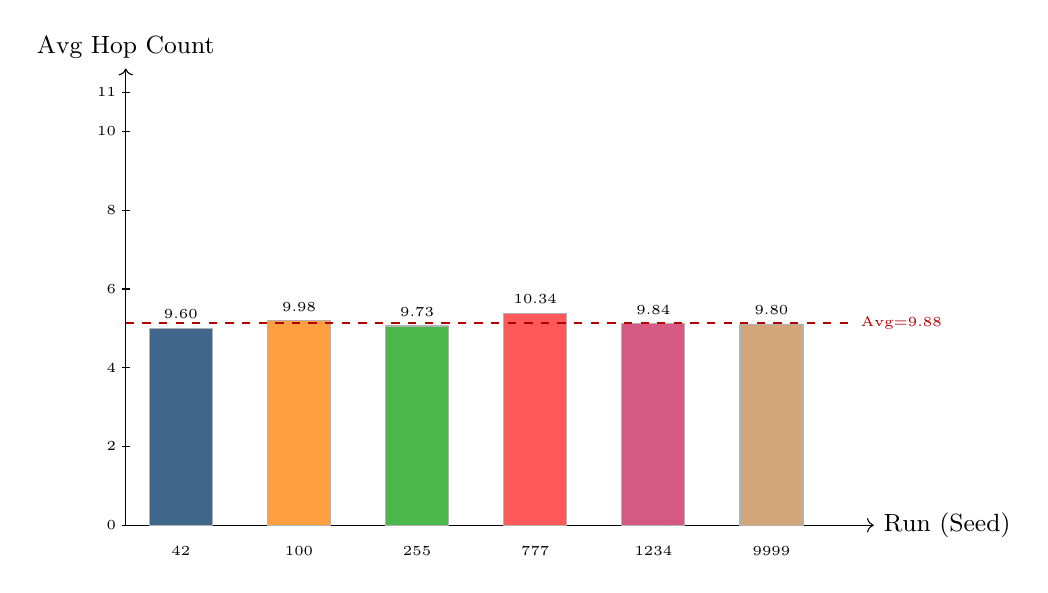
\begin{tikzpicture}
\begin{scope}
\draw[->] (0,0) -- (9.5,0) node[right]{\small Run (Seed)};
\draw[->] (0,0) -- (0,5.8) node[above]{\small Avg Hop Count};

\foreach \y/\val in {0/0, 1/2, 2/4, 3/6, 4/8, 5/10, 5.5/11} {
  \draw (-.05,\y) -- (.05,\y);
  \node[left,font=\tiny] at (0,\y) {\val};
}

\def\bw{0.8}
\def\sc{0.52}

\foreach \i/\label/\h/\col in {
  1/42/9.60/iiucblue!75,
  2/100/9.98/orange!75,
  3/255/9.73/green!60!black!70,
  4/777/10.34/red!65,
  5/1234/9.84/purple!65,
  6/9999/9.80/brown!70}
{
  \pgfmathsetmacro\xpos{0.3+(\i-1)*1.5}
  \pgfmathsetmacro\height{\h*\sc/2}
  \fill[\col] (\xpos,0) rectangle +(\bw,\height);
  \draw[gray!60, line width=0.4pt] (\xpos,0) rectangle +(\bw,\height);
  \node[font=\tiny,above] at (\xpos+\bw/2, \height) {\h};
  \node[font=\tiny,below] at (\xpos+\bw/2, -0.15) {\label};
}

% Overall avg line: 9.88 * 0.52/2 = 2.569
\draw[red!70!black, dashed, line width=1pt] (0,2.569) -- (9.2,2.569)
  node[right,font=\tiny,red!70!black] {Avg=9.88};
\end{scope}
\end{tikzpicture}
\caption{Average hop count per simulation run with overall average line}
\label{fig:barchart}
\end{figure}

\justifying
This figure shows that the average hop count per run ranges from 9.60 (Run 1, seed 42) to 10.34 (Run 4, seed 777). The dashed red line at 9.88 represents the overall average across all runs. The variation across seeds confirms that random routing produces non-deterministic path lengths, and no single seed consistently leads to shorter or longer paths.

\subsubsection{Hop Count Distribution: }

\begin{figure}[H]
\centering
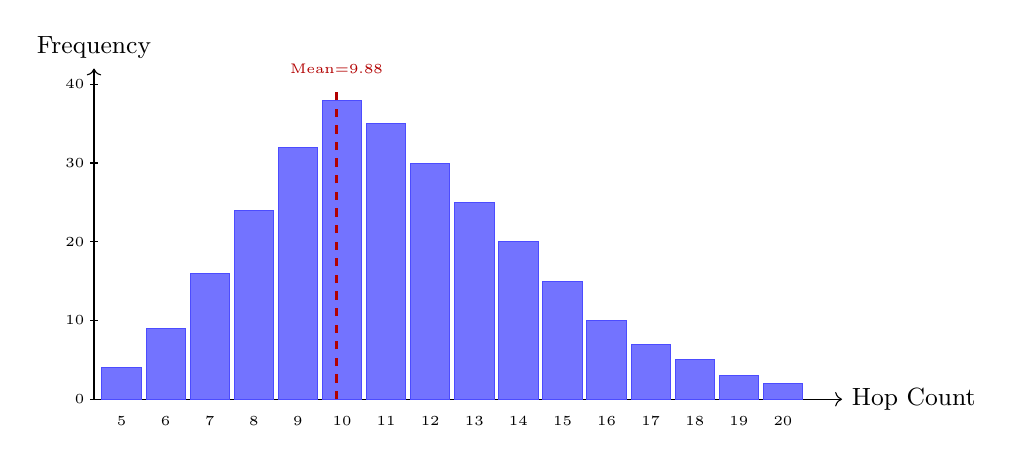
\begin{tikzpicture}
\draw[->] (0,0) -- (9.5,0) node[right]{\small Hop Count};
\draw[->] (0,0) -- (0,4.2) node[above]{\small Frequency};

\foreach \y in {0,1,2,3,4} {
  \draw (-.05,\y) -- (.05,\y);
  \node[left,font=\tiny] at (0,\y) {\pgfmathparse{int(\y*10)}\pgfmathresult};
}

% Histogram bars (approximate distribution: hops 5-20, peak ~8-12)
\foreach \i/\h in {
  1/0.4, 2/0.9, 3/1.6, 4/2.4, 5/3.2, 6/3.8,
  7/3.5, 8/3.0, 9/2.5, 10/2.0, 11/1.5, 12/1.0,
  13/0.7, 14/0.5, 15/0.3, 16/0.2}
{
  \pgfmathsetmacro\xpos{0.1+(\i-1)*0.56}
  \fill[blue!55] (\xpos,0) rectangle +(0.50,\h);
  \draw[blue!70, line width=0.3pt] (\xpos,0) rectangle +(0.50,\h);
  \pgfmathsetmacro\lab{int(\i+4)}
  \node[font=\tiny,below] at (\xpos+0.25,-0.10) {\lab};
}
% Mean line: 9.88 -> position ~(9.88-5)*0.56+0.35 = 3.08
\draw[red!70!black, dashed, line width=1pt] (3.08,0) -- (3.08,4.0)
  node[above,font=\tiny,red!70!black] {Mean=9.88};
\end{tikzpicture}
\caption{Approximate hop count frequency distribution across all 273 delivered packets}
\label{fig:distribution}
\end{figure}

\justifying
This figure illustrates the overall distribution of hop counts across all 273 delivered packets from six runs. The distribution is approximately bell-shaped with a peak around 9--11 hops, centered near the overall mean of 9.88. The spread from 5 to 20 hops reflects the randomness of path selection in the mesh topology.

\subsubsection{Received vs.\ Dropped Packets per Run: }

\begin{figure}[H]
\centering
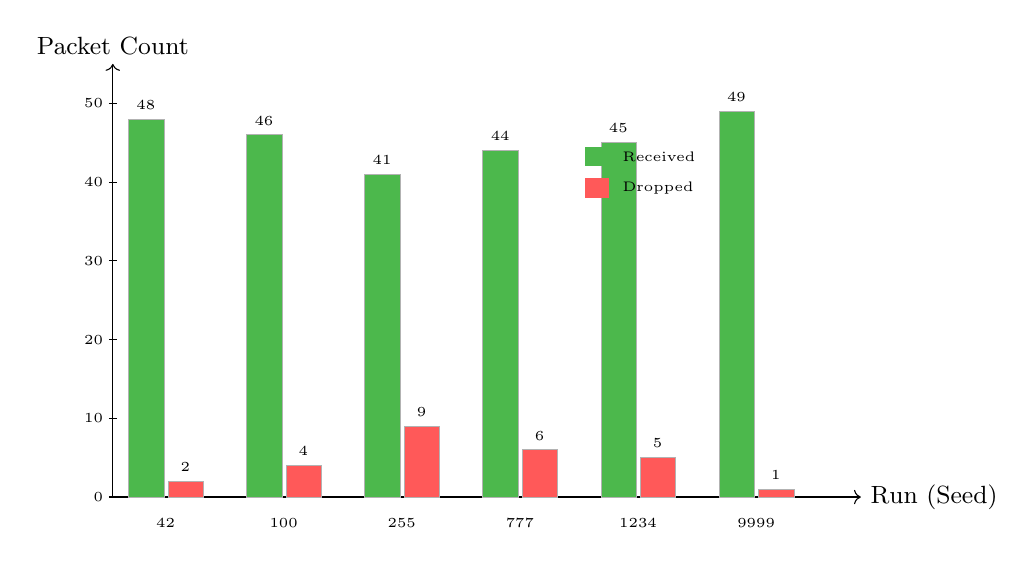
\begin{tikzpicture}
\draw[->] (0,0) -- (9.5,0) node[right]{\small Run (Seed)};
\draw[->] (0,0) -- (0,5.5) node[above]{\small Packet Count};

\foreach \y/\val in {0/0, 1/10, 2/20, 3/30, 4/40, 5/50} {
  \draw (-.05,\y) -- (.05,\y);
  \node[left,font=\tiny] at (0,\y) {\val};
}

% received bars (green) and dropped bars (red)
\foreach \i/\label/\recv/\drop in {
  1/42/48/2,
  2/100/46/4,
  3/255/41/9,
  4/777/44/6,
  5/1234/45/5,
  6/9999/49/1}
{
  \pgfmathsetmacro\xbA{0.2+(\i-1)*1.5}
  \pgfmathsetmacro\xbB{\xbA+0.5}
  \pgfmathsetmacro\hA{\recv*0.1}
  \pgfmathsetmacro\hB{\drop*0.1}
  \fill[green!60!black!70] (\xbA,0) rectangle +(0.45,\hA);
  \draw[gray!60, line width=0.3pt] (\xbA,0) rectangle +(0.45,\hA);
  \fill[red!65] (\xbB,0) rectangle +(0.45,\hB);
  \draw[gray!60, line width=0.3pt] (\xbB,0) rectangle +(0.45,\hB);
  \node[font=\tiny,below] at (\xbA+0.47,-0.15) {\label};
  \node[font=\tiny,above] at (\xbA+0.22,\hA) {\recv};
  \node[font=\tiny,above] at (\xbB+0.22,\hB) {\drop};
}

% Legend
\fill[green!60!black!70] (6.0,4.2) rectangle +(0.3,0.25);
\node[font=\tiny, right] at (6.35,4.32) {Received};
\fill[red!65] (6.0,3.8) rectangle +(0.3,0.25);
\node[font=\tiny, right] at (6.35,3.92) {Dropped};
\end{tikzpicture}
\caption{Received vs.\ dropped packets per simulation run}
\label{fig:recvdrop}
\end{figure}

\justifying
This figure compares the number of received (green) and dropped (red) packets for each run. Run 6 (seed 9999) achieved the best delivery performance with 49 received and only 1 dropped, while Run 3 (seed 255) had the worst performance with 9 dropped packets. The variation across seeds is entirely due to different random routing paths chosen by \texttt{intuniform()}.

% ══════════════════════════════════════════════════════════════════
%  SECTION 11 — SCREENSHOT SECTION
% ══════════════════════════════════════════════════════════════════
\section{Screenshot Section: }


\begin{center}

\includegraphics[width=0.7\textwidth]{screenshot/sim.png}


{\small \textbf{Figure 4:} After running the simulations in OMNeT++}

\end{center}



\subsection{OMNeT++ Network Topology View: }

\begin{figure}[H]
\centering
{\begin{minipage}{0.9\textwidth}
\centering
\includegraphics[width=0.5\textwidth]{screenshot/mesh.png}



{\small \textbf{Figure 5:} Network topology visualization in OMNeT++ 6 IDE.}
\end{minipage}}
\caption{This figure shows the complete mesh network layout rendered by the simulator, with labeled nodes and directed link arrows connecting the Sender through routers r0--r9 to the Receiver.}
\end{figure}

\subsection{Simulation Run Event Log: }

\begin{figure}[H]
\centering
{\begin{minipage}{0.9\textwidth}
\centering
\includegraphics[width=0.7\textwidth]{screenshot/event.png}



{\small \textbf{Figure 6:} Simulation event log output during Run1.}
\end{minipage}}
\caption{This figure displays the console EV log showing each router's name, the current hopCount and TTL values after processing each packet, and the Receiver's final arrival confirmation with statistics.}
\end{figure}

\subsection{Python Analysis Output Chart: }

\begin{figure}[H]
\centering
{\begin{minipage}{0.9\textwidth}
\centering

\includegraphics[width=1.1\textwidth]{screenshot/hop_count_analysis.png}
{\small \textbf{Figure 7:} {hop\_count\_analysis.png} generated by the Python analysis script.}
\end{minipage}}
\caption{This figure presents the complete visualization output: the bar chart shows average hop counts per seed with the overall mean marked in red, the histogram reveals the distribution shape of hop counts across all 273 deliveries, and the grouped bar chart compares received versus dropped packets per run.}
\end{figure}

% ══════════════════════════════════════════════════════════════════
%  SECTION 12 — DISCUSSION
% ══════════════════════════════════════════════════════════════════
\section{Discussion: }

\justifying
The simulation results reveal several important characteristics of random routing in mesh networks:

\textbf{Path Length Variability:} The average hop count per run ranged from 9.60 to 10.34, and individual packet hop counts ranged from 5 to 20. This demonstrates that random routing produces significantly variable path lengths even across packets in the same run and the same topology. The variability arises because \texttt{intuniform()} at each router can lead a packet through a short direct path or a long circuitous route through r9's back-connections to r6 and r7.

\textbf{TTL Effectiveness:} The overall drop rate was 9\% (27 out of 300 packets). While the TTL of 20 was sufficient for the majority of packets, the directed graph cycles (r9 $\to$ r6 or r7 $\to$ r9 again) allow some packets to loop multiple times before either reaching the Receiver or being dropped. Increasing TTL to 30 would likely reduce the drop rate further, while decreasing it would increase drops.

\textbf{Seed-Dependent Performance:} Run 6 (seed 9999) delivered 49 out of 50 packets (98\%), while Run 3 (seed 255) delivered only 41 (82\%). This significant seed-dependent variation highlights that a single simulation run is insufficient for reliable network analysis; multiple seeds are necessary to obtain statistically meaningful results.

\textbf{Mesh Topology and Connectivity:} The rich connectivity of the 10-router mesh (with each router having 2--4 outgoing connections) ensures packets almost always have multiple forwarding options. However, the presence of directed cycles can cause packets to revisit routers, inflating hop counts and increasing the probability of TTL expiry on certain seeds.

% ══════════════════════════════════════════════════════════════════
%  SECTION 13 — CONCLUSION
% ══════════════════════════════════════════════════════════════════
\section{Conclusion: }

\justifying
The outcomes of this laboratory experiment are summarized as follows:

\begin{enumerate}

\item The hop counting system was successfully implemented in a random mesh network using OMNeT++.

\item Routers correctly increased the \texttt{hopCount} value and decreased the \texttt{ttl} value during packet forwarding.

\item Random routing created different hop counts for different packets and simulation runs.

\item The TTL mechanism successfully prevented infinite routing loops by dropping expired packets.

\item The Python analysis script calculated average hop count, dropped packets, and generated graphical results automatically.

\item This experiment improved practical knowledge of OMNeT++, network simulation, routing concepts, and result analysis using Python.

\end{enumerate}

\vspace{7.0cm}
\noindent\textcolor{iiucblue}{\rule{\linewidth}{0.6pt}}
\vspace{0.3cm}
\begin{center}
{\small \textit{Department of Computer Science \& Engineering, IIUC}
\quad $\bullet$ \quad
\textit{CSE-4834: Computer Networks Lab}}
\end{center}

\end{document}